\documentclass[10pt, a5paper]{article}
\usepackage{pdfpages}
\usepackage{parallel}
\usepackage[T2A]{fontenc}
\usepackage{ucs}
\usepackage[utf8x]{inputenc}
\usepackage[polish,english,russian]{babel}
\usepackage{hyperref}
\usepackage{rotating}
\usepackage[inner=2cm,top=1.8cm,outer=2cm,bottom=2.3cm,nohead]{geometry}
\usepackage{listings}
\usepackage{graphicx}
\usepackage{wrapfig}
\usepackage{longtable}
\usepackage{indentfirst}
\usepackage{array}
\newcolumntype{P}[1]{>{\raggedright\arraybackslash}p{#1}}
\frenchspacing
\usepackage{fixltx2e} %text sub- and superscripts
\usepackage{icomma} % коскі ў матэматычным рэжыме
\PreloadUnicodePage{4}

\newcommand{\longpage}{\enlargethispage{\baselineskip}}
\newcommand{\shortpage}{\enlargethispage{-\baselineskip}}

\def\switchlang#1{\expandafter\csname switchlang#1\endcsname}
\def\switchlangbe{
\let\saverefname=\refname%
\def\refname{Літаратура}%
\def\figurename{Іл.}%
}
\def\switchlangen{
\let\saverefname=\refname%
\def\refname{References}%
\def\figurename{Fig.}%
}
\def\switchlangru{
\let\saverefname=\refname%
\let\savefigurename=\figurename%
\def\refname{Литература}%
\def\figurename{Рис.}%
}

\hyphenation{admi-ni-stra-tive}
\hyphenation{ex-pe-ri-ence}
\hyphenation{fle-xi-bi-li-ty}
\hyphenation{Py-thon}
\hyphenation{ma-the-ma-ti-cal}
\hyphenation{re-ported}
\hyphenation{imp-le-menta-tions}
\hyphenation{pro-vides}
\hyphenation{en-gi-neering}
\hyphenation{com-pa-ti-bi-li-ty}
\hyphenation{im-pos-sible}
\hyphenation{desk-top}
\hyphenation{elec-tro-nic}
\hyphenation{com-pa-ny}
\hyphenation{de-ve-lop-ment}
\hyphenation{de-ve-loping}
\hyphenation{de-ve-lop}
\hyphenation{da-ta-ba-se}
\hyphenation{plat-forms}
\hyphenation{or-ga-ni-za-tion}
\hyphenation{pro-gramming}
\hyphenation{in-stru-ments}
\hyphenation{Li-nux}
\hyphenation{sour-ce}
\hyphenation{en-vi-ron-ment}
\hyphenation{Te-le-pathy}
\hyphenation{Li-nux-ov-ka}
\hyphenation{Open-BSD}
\hyphenation{Free-BSD}
\hyphenation{men-ti-on-ed}
\hyphenation{app-li-ca-tion}

\def\progref!#1!{\texttt{#1}}
\renewcommand{\arraystretch}{2} %Іначай формулы ў матрыцы зліпаюцца з лініямі
\usepackage{array}

\def\interview #1 (#2), #3, #4, #5\par{

\section[#1, #3, #4]{#1 -- #3, #4}
\def\qname{LVEE}
\def\aname{#1}
\def\q ##1\par{{\noindent \bf \qname: ##1 }\par}
\def\a{{\noindent \bf \aname: } \def\qname{L}\def\aname{#2}}
}

\def\interview* #1 (#2), #3, #4, #5\par{

\section*{#1\\{\small\rm #3, #4. #5}}

\def\qname{LVEE}
\def\aname{#1}
\def\q ##1\par{{\noindent \bf \qname: ##1 }\par}
\def\a{{\noindent \bf \aname: } \def\qname{L}\def\aname{#2}}
}

\switchlang{en}
\begin{document}
\title{Running MySQL in Kubernetes}
\author{Mykola Marzhan, Kyiv, Ukraine; \\ Dmitriy Kostiuk, Brest, Belarus\footnote{\url{delgod@delgod.com}, \url {https://lvee.org/ru/abstracts/309}} }
\maketitle
\begin{abstract}
Running databases in Kubernetes attracts a lot of attention today. Orсhestration of MySQL on Kubernetes is no way a \linebreak straightforward process. There are several good MySQL based solutions in the open-source world, made by Oracle, Presslabs, and Percona. Having a common base, they differ in self-healing capabilities, multimaster and backup/restore support, etc. So let’s make a fair comparison to figure out the pros and cons of their current state.
\end{abstract}
Without question, Kubernetes is the most popular container \linebreak orchestration platform, and container orchestration itself is an excellent approach for packaging and deployment, which allows you to deploy a known version of configuration, code, environment in a deterministic way.

In general, databases easiest for containerization are those which manage their state and make themselves effectively stateless from the point of the scheduler and container orchestration, i.e. ones that provide cluster membership, fault-tolerance, and data replication. Databases that do not do these things on their own require additional services and/or application-specific frameworks to operate reliably.

Thus, deploying MySQL in containerized environment turns out to be a rather complicated task, which involves additional components and their setup. Most known MySQL based solutions for Kubernetes in the open-source world are made by Presslabs \cite{bib1}, Percona \cite{bib2}, and Oracle \cite{bib3}, and all three are based on a specially developed Kubernetes Operator.

Kubernetes Operator extends the Kubernetes API with a new \linebreak custom resource for deploying, configuring, and managing the application through the whole life cycle. You can compare the Kubernetes Operator to a System Administrator who deploys the application and watches the Kubernetes events related to it, taking administrative/ operational actions when needed.

It allows you to launch a new environment with no single point of failure in under 10 minutes, and will reliably orchestrate scaling the environment to meet current requirements if needed, adding or removing nodes quickly and efficiently. Kubernetes Operators also provides self-healing of a failed node in a cluster environment.

The Presslabs MySQL Operator \cite{bib1} has the most simple architecture -- regular MySQL asynchronous replication, with backups support (both scheduled and on-demand ones), and high availability of the database cluster. The operator is still in its alpha stage. HA features are based on the orchestrator project \cite{bib4}, and also, the monitoring capabilities are provided with the use of Prometheus time-series database \cite{bib5}.

Percona Kubernetes Operator for XtraDB Cluster \cite{bib2} is a Percona solution for managing the Percona XtraDB Cluster deployment in a Kubernetes or OpenShift environment, which also officially supports Minikube. Percona XtraDB Cluster in its turn is a database clustering solution that integrates Percona Server for MySQL running with the XtraDB storage engine, and Percona XtraBackup with the Galera \linebreak library to enable synchronous multi-master replication. Percona XtraDB Cluster also includes ProxySQL for load balancing. The Operator also adds Percona Monitoring and Management \cite{bib6} to provide you with deep visibility into the performance and usage of the cluster \cite{bib7}.

The design of the operator is bound to the Percona XtraDB Cluster, but the following diagram shows how it is related to the Kubernetes resources and is similar to all MySQL operators:

\begin{center}
\begin{figure}[h!]
  \centering
  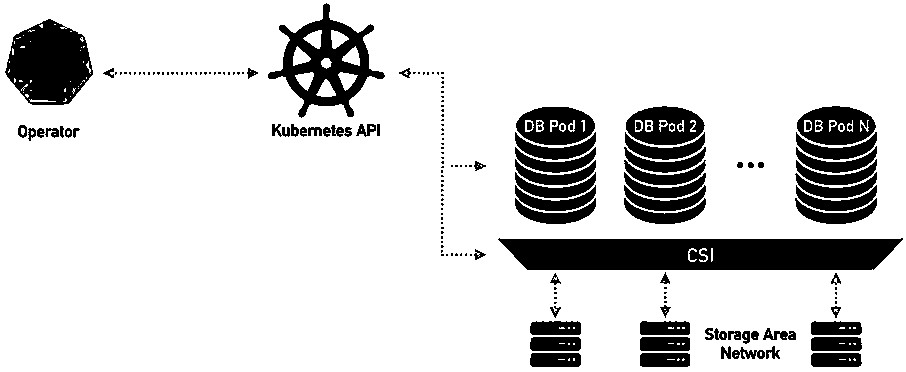
\includegraphics[width=11cm]{19_2019_Marzhan.jpg}
  %\caption{Statue of Liberty}	
  \label{fig1}
\end{figure}
\end{center}

To provide high availability operator uses node affinity to run PXC instances on separate worker nodes, with the automatical re-creation of the failed container on another node. Scheduled and on-demand backups can be done on any S3-compatible storage or stored locally. The operator also uses TLS cryptographic protocol as for internal communications (between PXC instances in the cluster) and external ones (between the client application and ProxySQL).

The MySQL Operator from Oracle uses a similar approach and is based on MySQL InnoDB Cluster \cite{bib3}. It provides scheduled and on-demand backups and restore, and uses Kubernetes Persistent Volume Claims to store data on local disk or network-attached storage. It is also able to use Prometheus to gather monitoring metrics.

\begin{thebibliography}{9}
\bibitem{bib1} presslabs/mysql-operator: Bulletproof MySQL on Kubernetes using Percona Server \url{https://github.com/presslabs/mysql-operator}
\bibitem{bib2} percona/percona-xtradb-cluster-operator: Percona Kubernetes Operator for XtraDB Cluster \url{https://github.com/percona/percona-xtradb-cluster-operator}
\bibitem{bib3} oracle/mysql-operator: Create, operate and scale self-healing MySQL clusters in Kubernetes \url{https://github.com/oracle/mysql-operator}
\bibitem{bib4} github/orchestrator: MySQL replication topology management and HA. \url{https://github.com/github/orchestrator}
\bibitem{bib5} Prometheus -- Monitoring system \& time-series database. \url{https://prometheus.io/}
\bibitem{bib6} Percona Monitoring and Management Documentation \url{https://www.percona.com/doc/percona-monitoring-and-management}
\bibitem{bib7} Percona XtraDB Cluster 5.7 Documentation \url{https://www.percona.com/doc/percona-xtradb-cluster}
\end{thebibliography}
\end{document}
